% Software Development for Mobile Devices
\documentclass[11pt,english,numbers=endperiod,parskip=half]{scrartcl}

\usepackage{color}
\usepackage{graphicx}
\usepackage{minted}
\usepackage{fancyhdr}

\pagestyle{fancy}

\rhead{Daniel Parker - 971328X}
\lhead{COS30017 - Software Development for Mobile Devices}

\title{Assignment 02}
\subtitle{COS30017 - Software Development for Mobile Devices}
\author{Daniel Parker 971328X}

\date{\today}

\begin{document}
\maketitle
\thispagestyle{empty}

\section{Task 1}
\subsection{Orientation Changes}
\raggedright
When the device orientation changes, a certain sequence of steps is being followed by the activity's lifecycle. Before the orientation of the device changes the activity is running, once the phone has been turned to it's side the activity moves to \textit{onPause()} then \textit{onStop()} and then \textit{onDestroy()}. The activity is then created again at \textit{onCreate()} with the new orientation and follows the lifecycle from there onwards as usual. \bigskip \\

\setlength\fboxsep{0pt}
\setlength\fboxrule{0.5pt}
\centering{
	\fbox{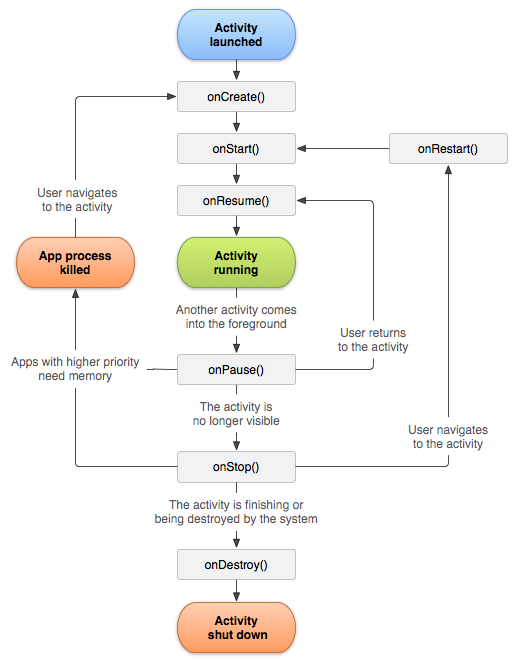
\includegraphics[width=7cm]{images/activity_lifecycle.png}}
}\\
\bigskip
\centering{
	\fbox{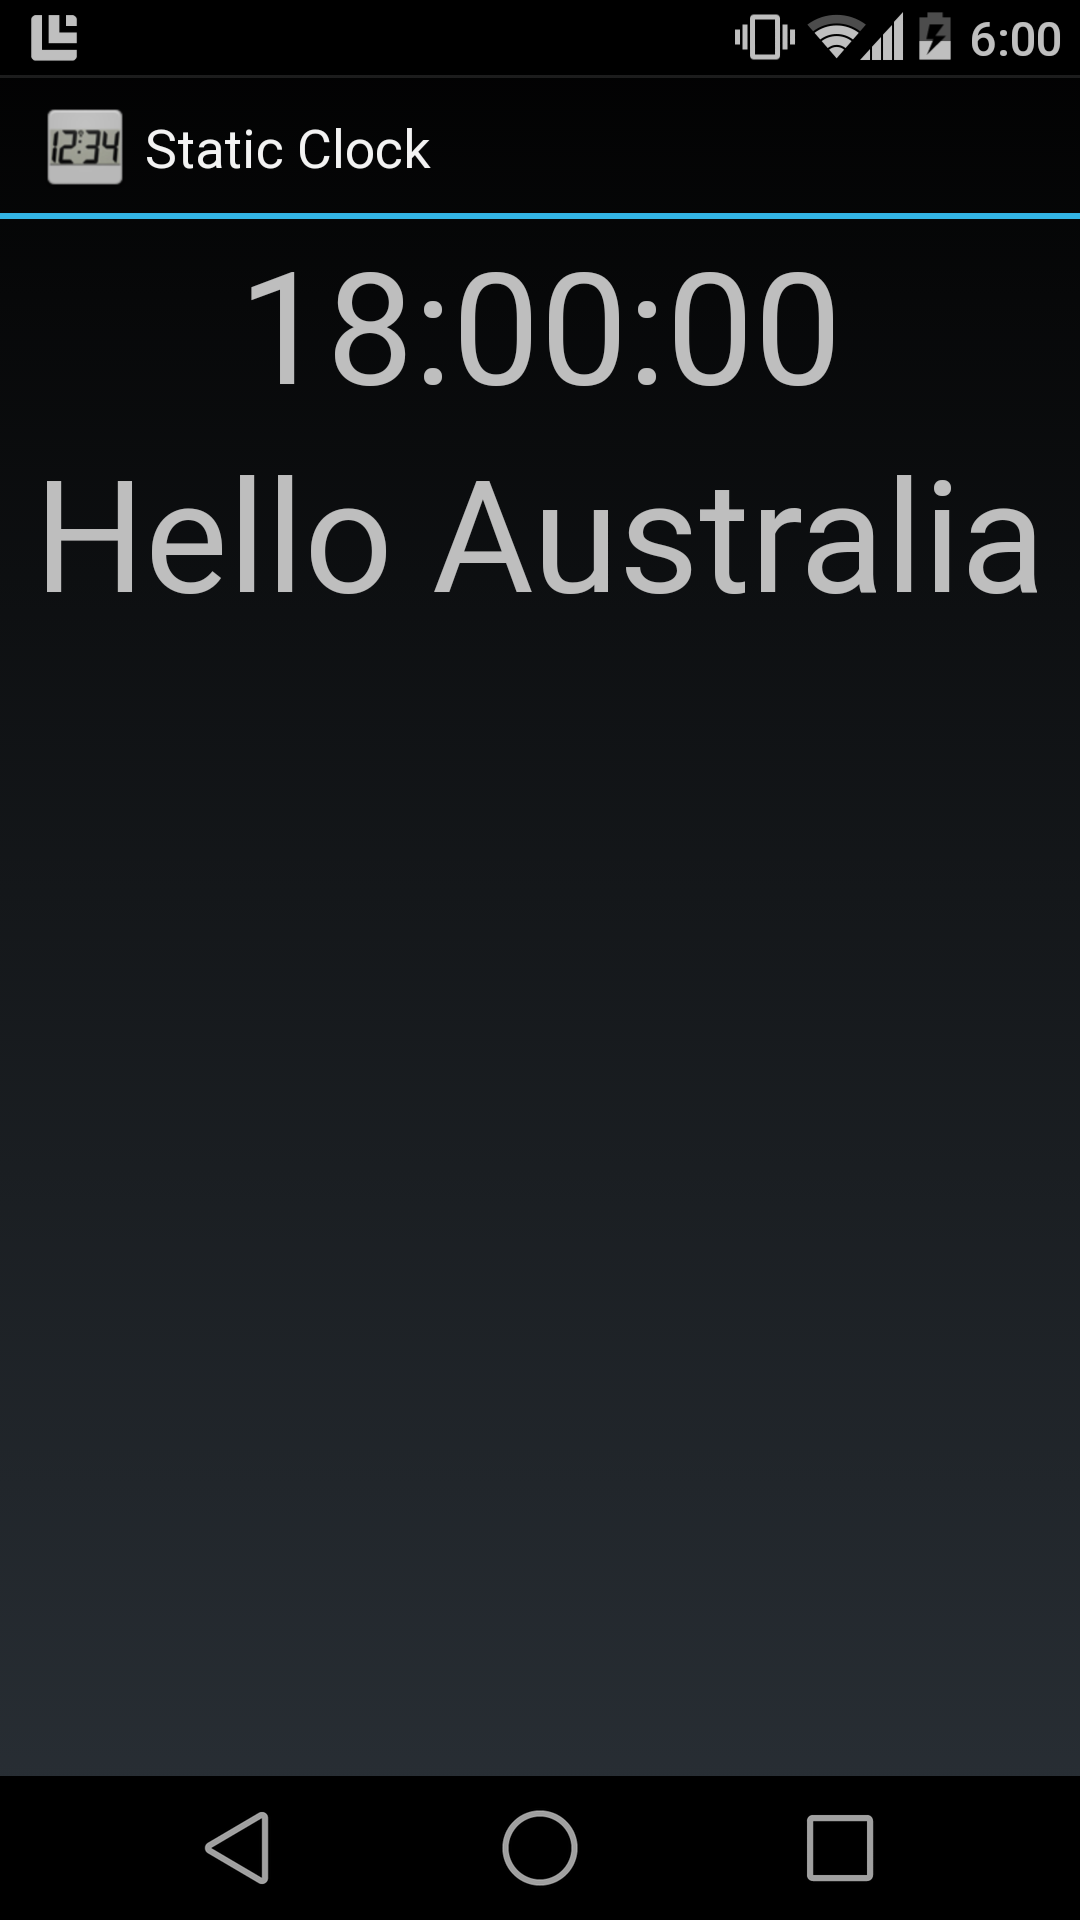
\includegraphics[width=5cm]{images/screenshot-portrait-1.png}}
}\\
\bigskip
\centering{
	\fbox{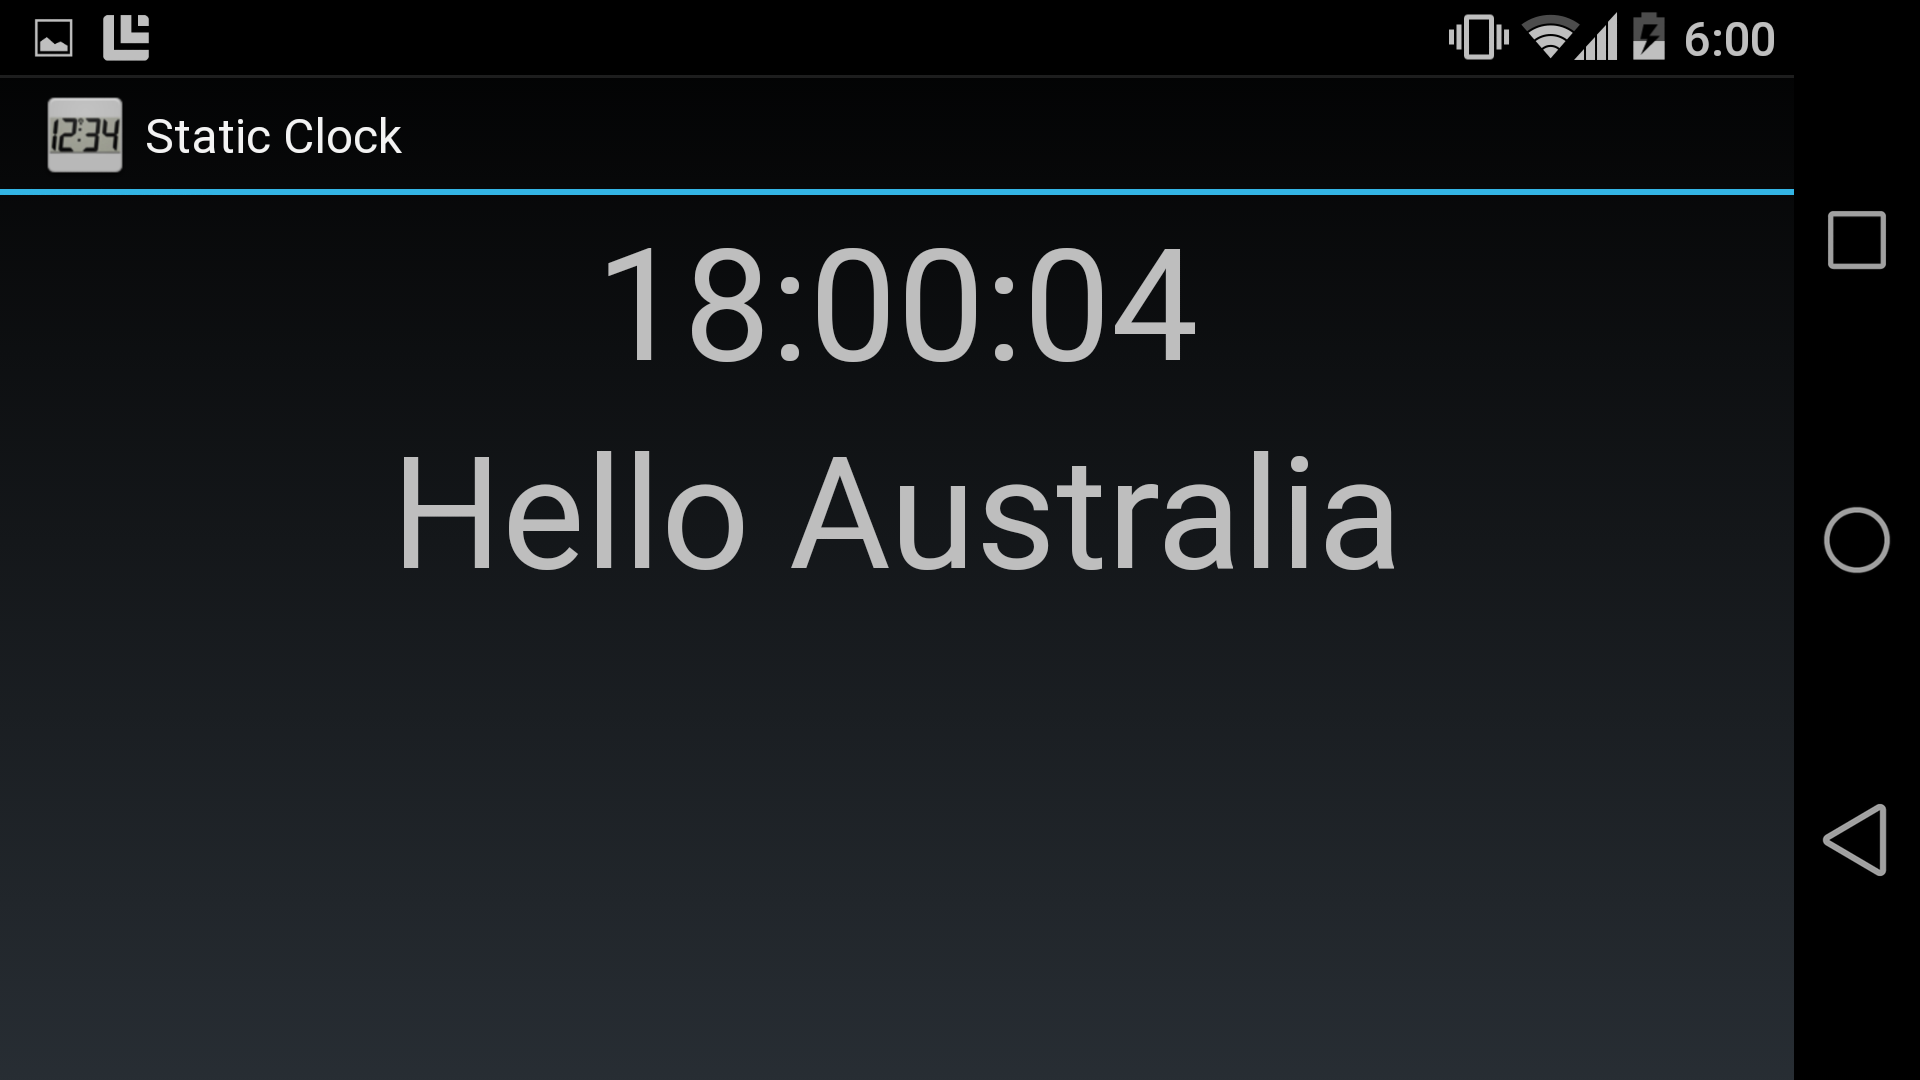
\includegraphics[width=10cm]{images/screenshot-landscape-1.png}}
}\\
\bigskip
\raggedright
We observe a time change after the orientation change because when the activity is destroyed and then recreated at \textit{onCreate()} the actual time is updated to the time at which it was recreated.
\subsection{Resume, Pause and Stop States}
The \textit{Pause} state is entered when the user navigates away from the specific activity by clicking a settings button (thus entering another activity) or otherwise. The activity has not been destroyed it has just moved into the pause state.

When the user navigates back to the activity within the app, the activity will then enter the \textit{Resume} state to prepare for the user to start using it again. This transition happens most commonly when the back button is pressed within an app and the activity comes back into the foreground.

If the user exits the activity either by navigating away from the app or returning to a previous activity then this activity will enter the \textit{Stop} state once it is no longer visible. The activity will pass the \textit{Pause} state on it's way to this state.

\section{Task 2}
As shown in the screenshot below, the \textit{onRestart()} event can be triggered. This was done by pressing the 'Home' button and then navigating back to the app using the app drawer.

\centering{
	\fbox{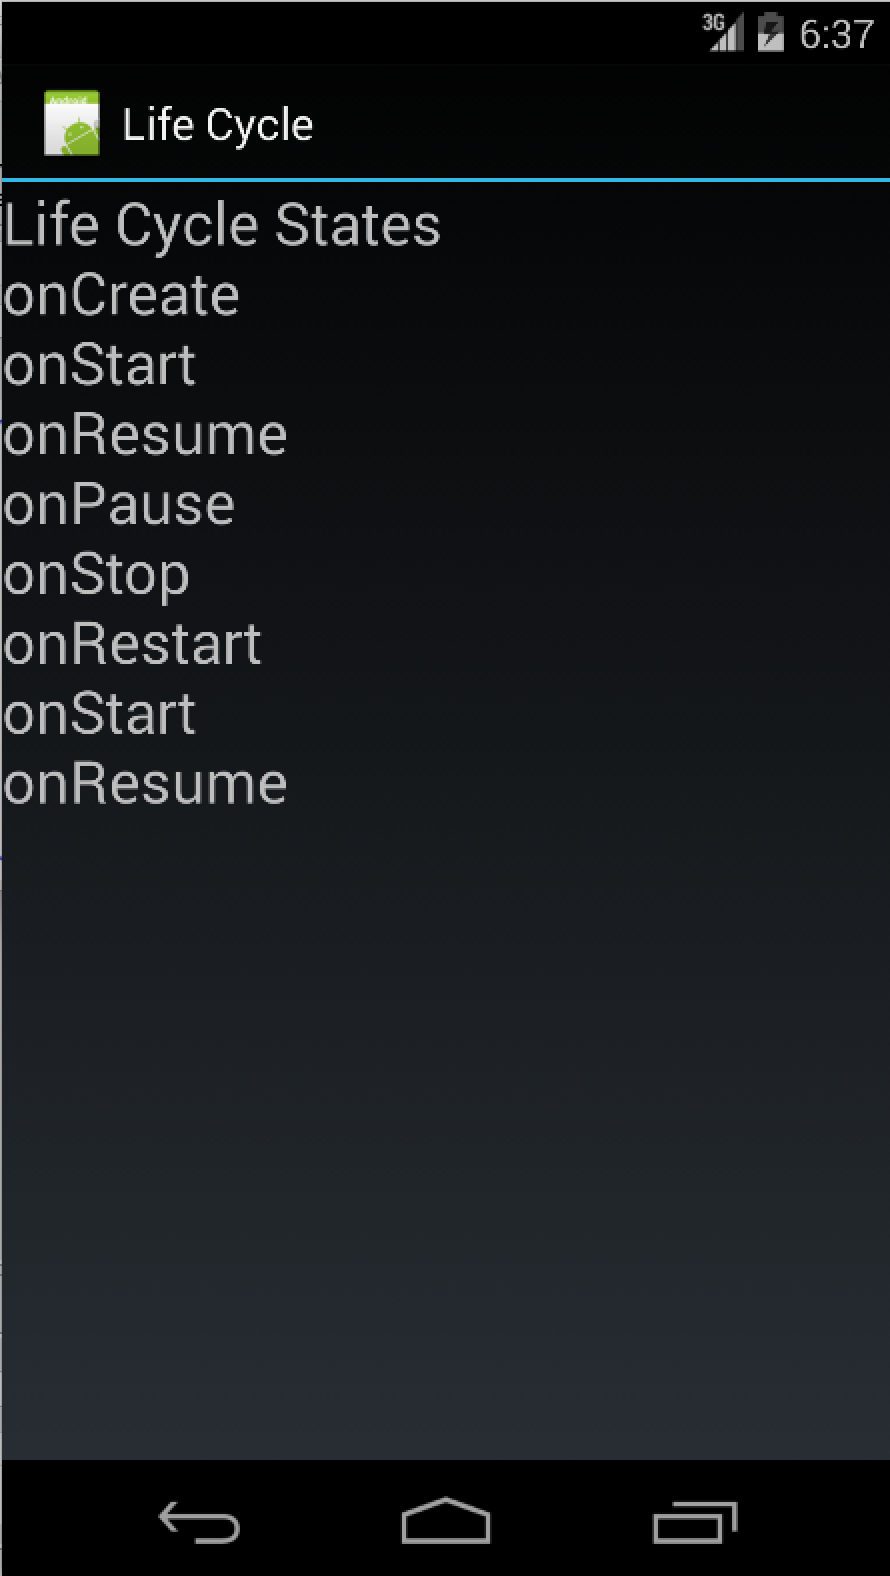
\includegraphics[width=7cm]{images/screenshot-states.png}}
}\\
\bigskip

\section{Task 3}
\raggedright
Invoking all the different lifecycle states we can see those that are printible in the activity normally, however the \textit{onDestroy()|} state never gets printed to the activity because the activity is no longer visible on the screen when the state occurs and due to the activity being destroyed the text won't be visible when the activity starts again because the data is lost.

\centering{
\fbox{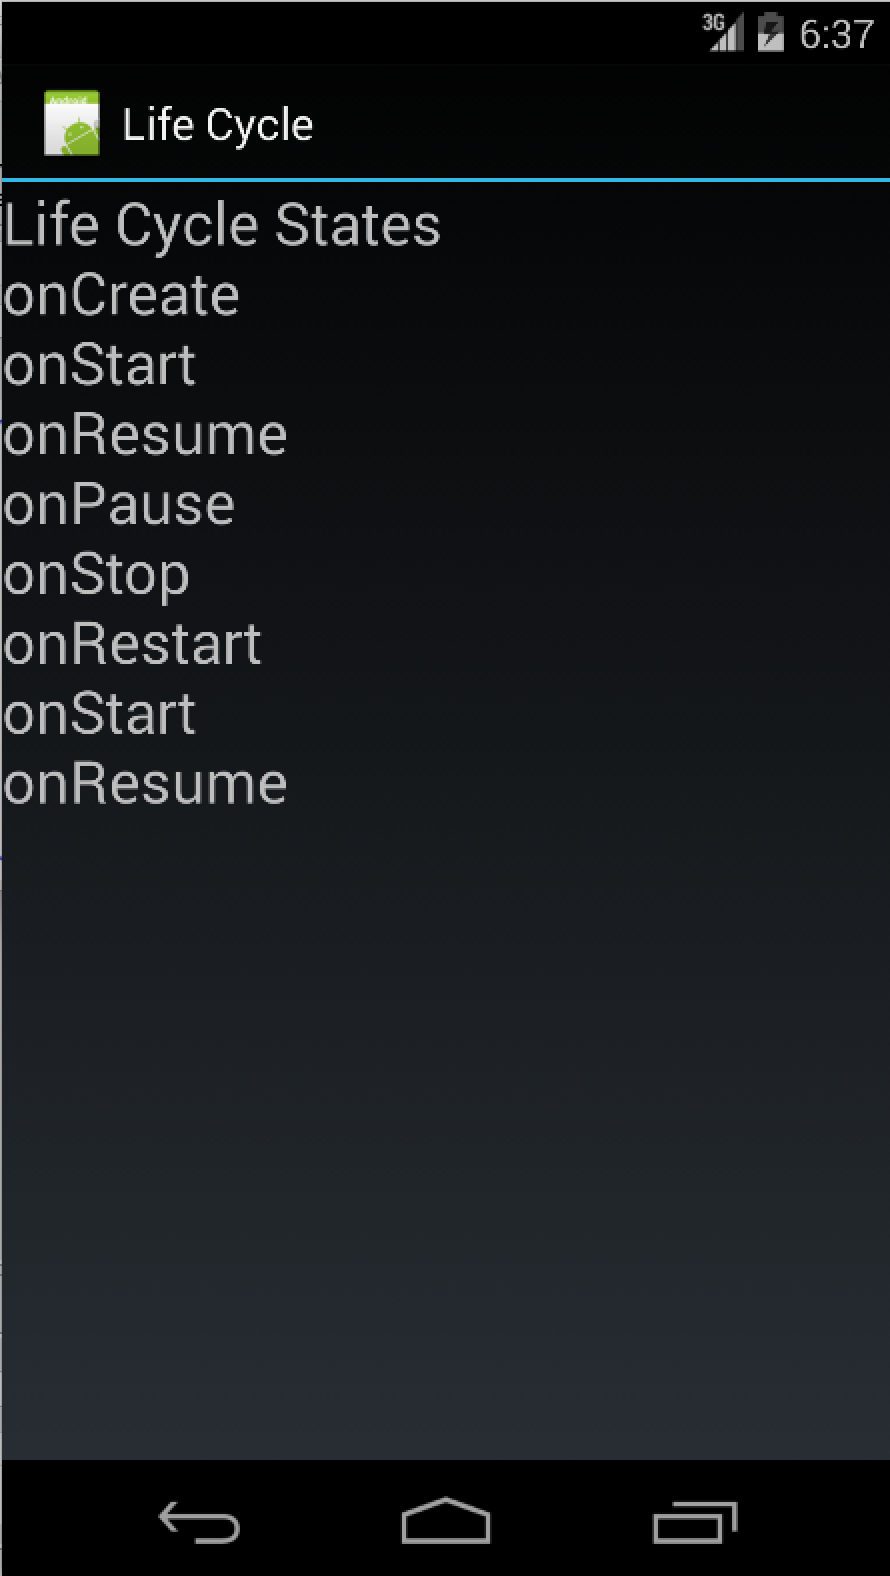
\includegraphics[width=7cm]{images/screenshot-states.png}}
}\\
\bigskip

The following screenshots show the logcat messages for when each state is reached.
\bigskip
\centering{
\fbox{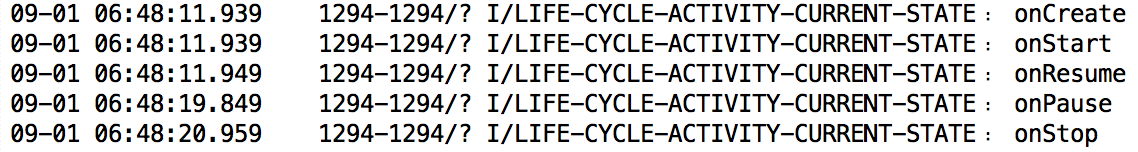
\includegraphics[width=12cm]{images/screenshot-logcat-1.png}}
}\\
\bigskip
\centering{
	\fbox{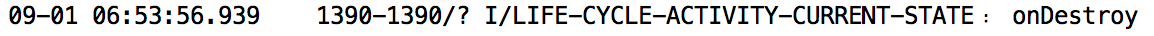
\includegraphics[width=12cm]{images/screenshot-logcat-2.png}}
}\\
\bigskip

\section{Task 4}
\raggedright
String externalisation allows us to supply different language strings for the same reference string. For example in this Hello, World! program there is an English strings.xml and a Spanish strings.xml. The Android convention puts them in two different values directories within \textit{res}. The English strings.xml are just in the normal \textit{values} directory, and the Spanish strings.xml are in the \textit{values-es} directory which is short for \textit{Espanol}.

\bigskip
\centering{
	\fbox{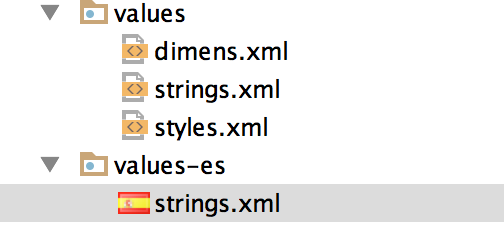
\includegraphics[width=6cm]{images/screenshot-values.png}}
}\\
\bigskip
\centering{
	\fbox{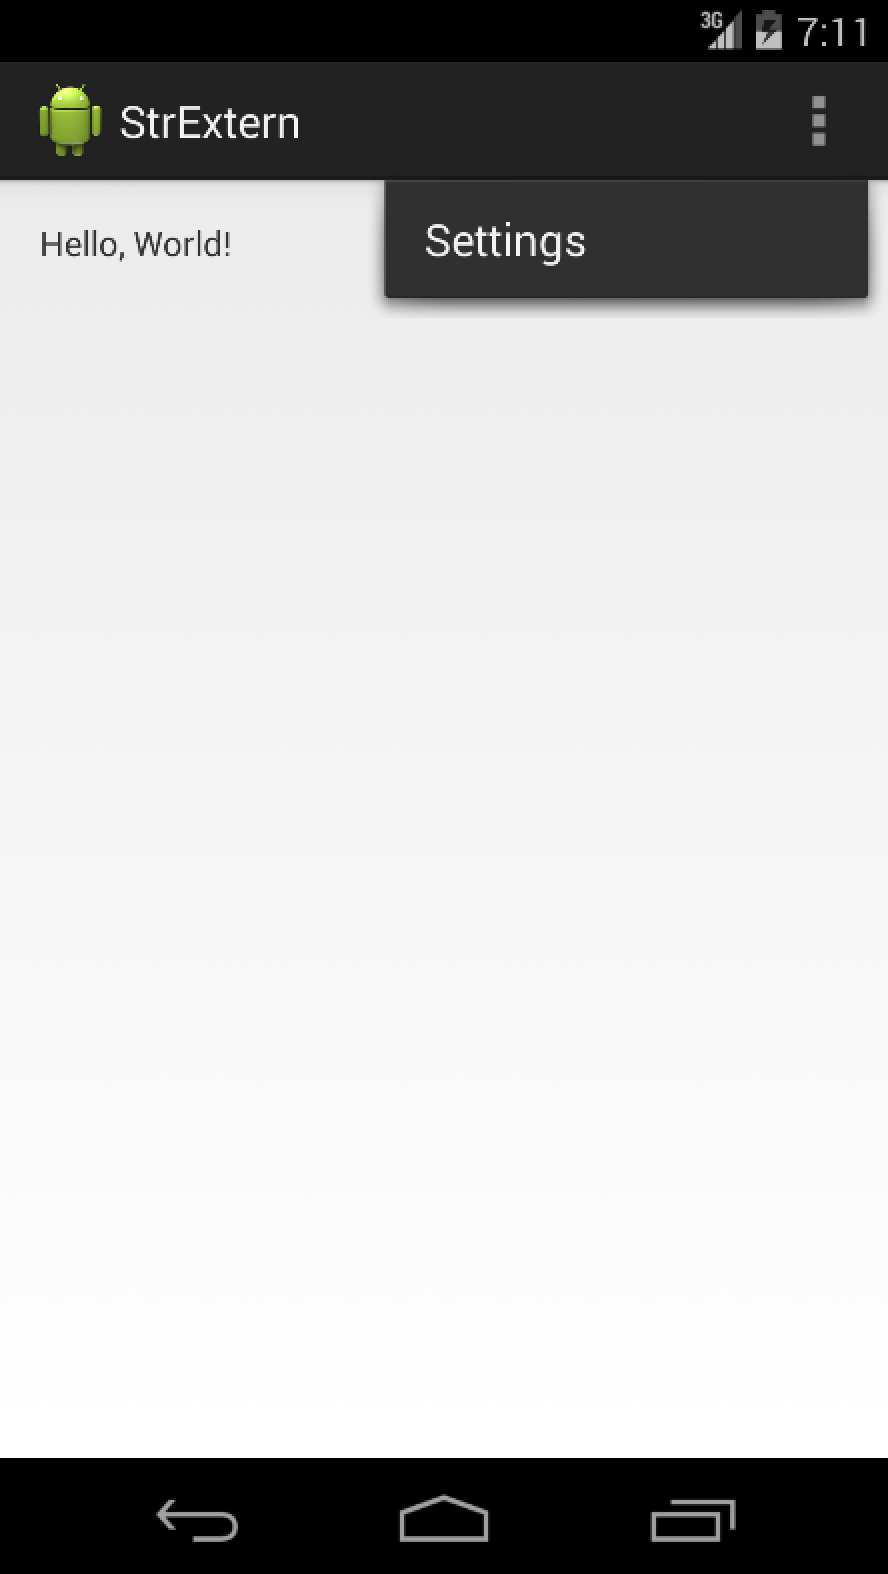
\includegraphics[width=6cm]{images/screenshot-english.png}}
}\\
\bigskip
\centering{
	\fbox{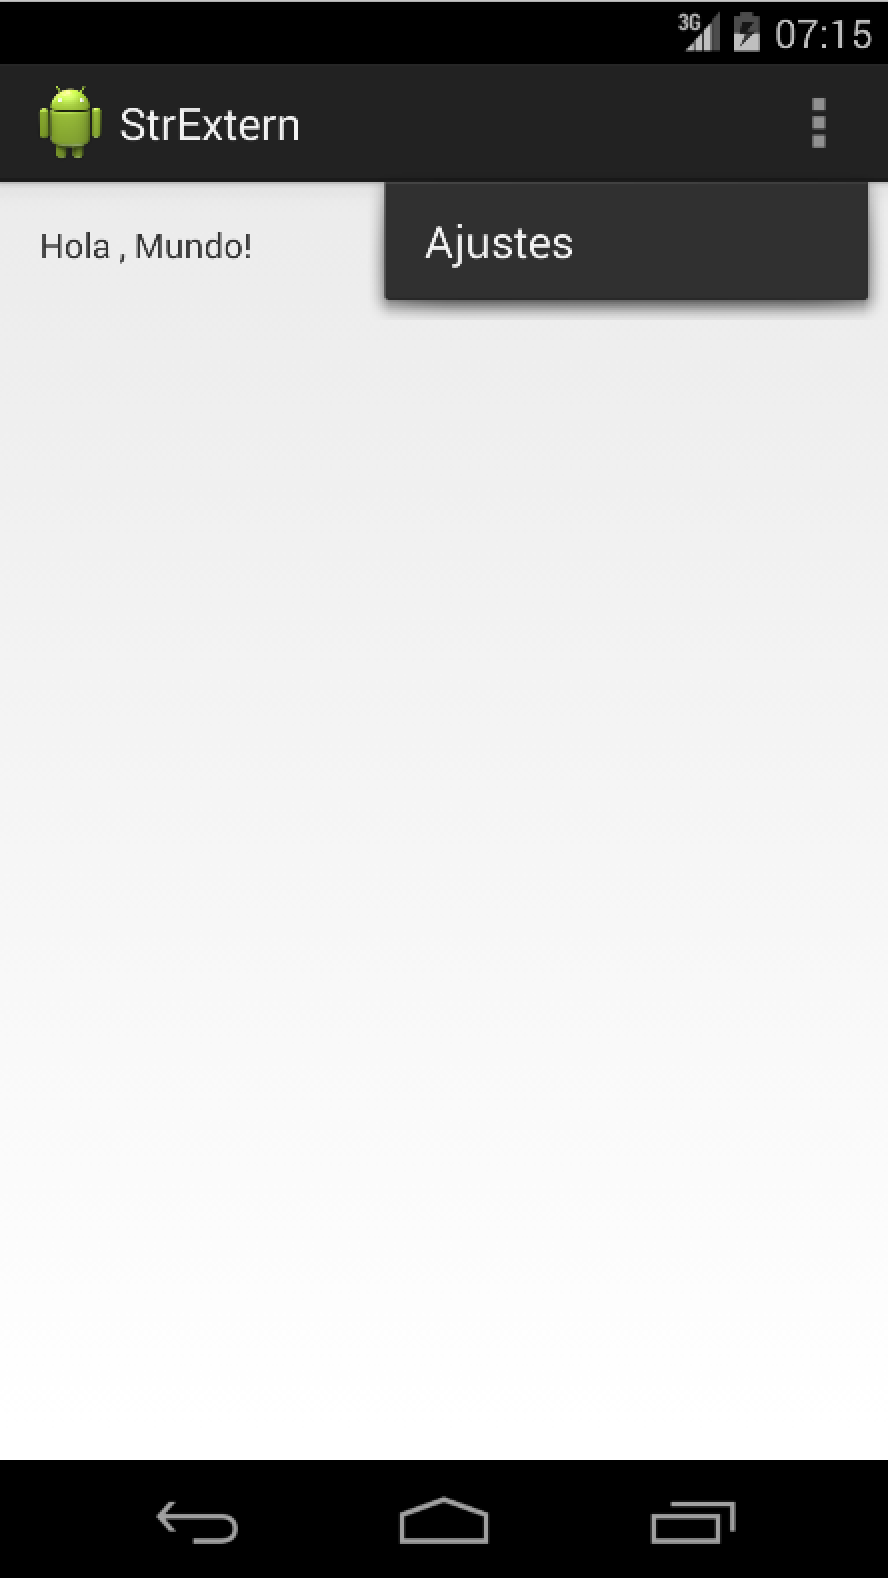
\includegraphics[width=6cm]{images/screenshot-spanish.png}}
}\\
\bigskip

\subsection{Source}
\inputminted{xml}{../../Apps/StrExtern/app/src/main/res/layout/activity_main.xml}

\section{Task 5}
\raggedright
In this application, the landscape activity will use it's own layout supplied in the \textit{layout-land} directory. When the orientation changes to landscape that will be the layout used. The difference with this layout is that the whole activity is enclosed within a ScrollView so that the user can scroll down and access the lower parts of the activity. 

When a user enters a height larger than 8 foot (or 96 inches) the app will display a toast to say that they are suspiciously tall for a human. This can be seen in the third screenshot. When the user checks the checkbox, and then clicks the \textit{Convert} button, the answer will be given in metres instead of centimetres.
\subsection{Screenshots}
\centering{
	\fbox{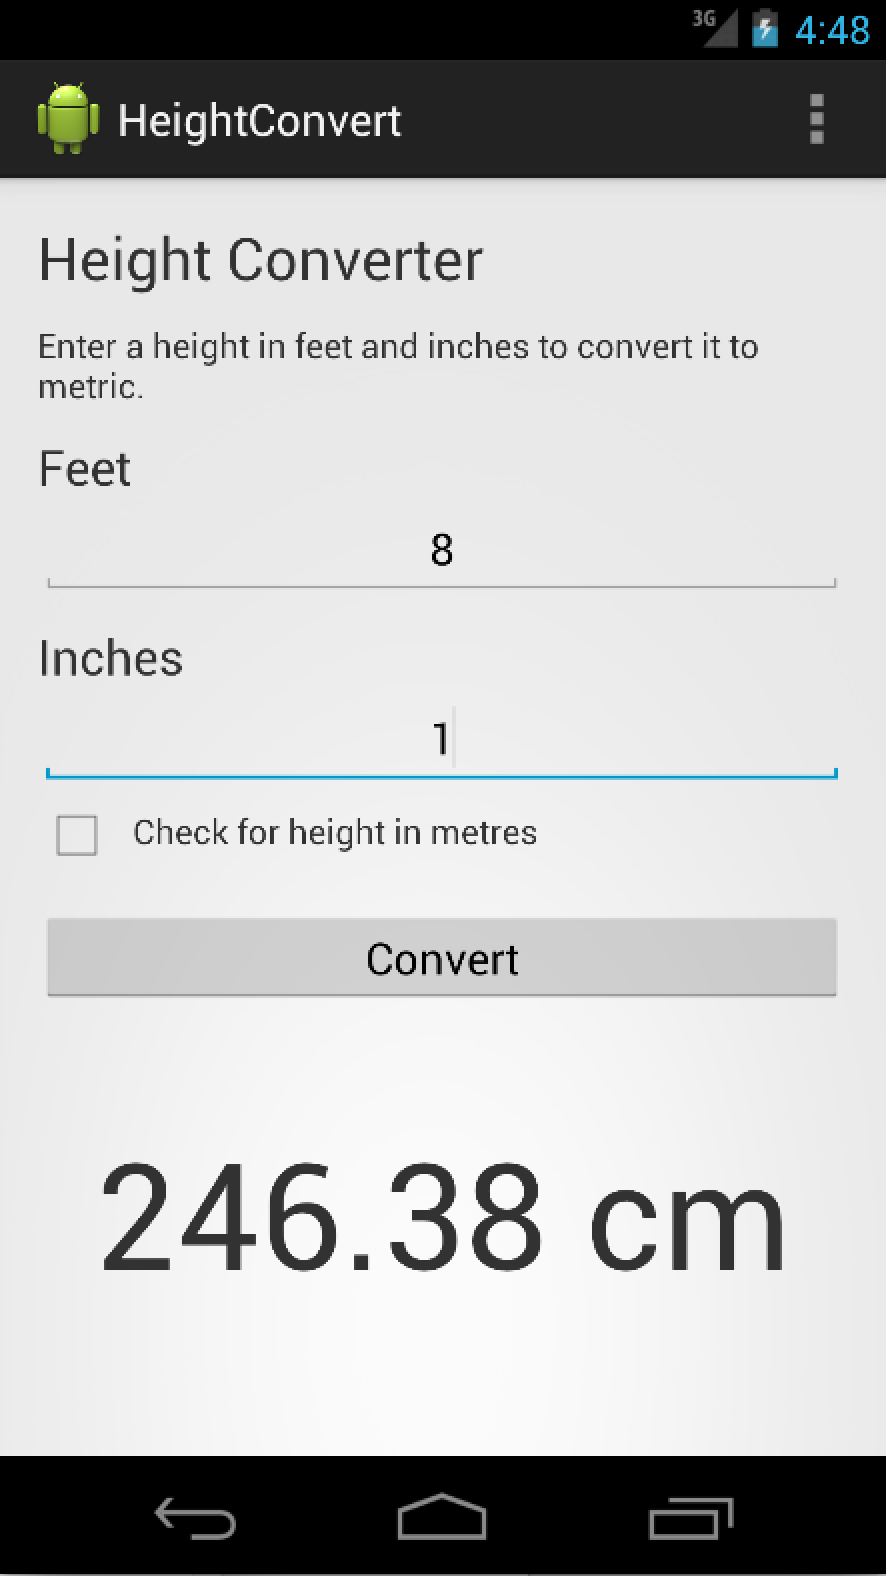
\includegraphics[width=6cm]{images/screenshot-height-portrait.png}}
}\\
\bigskip
\centering{
	\fbox{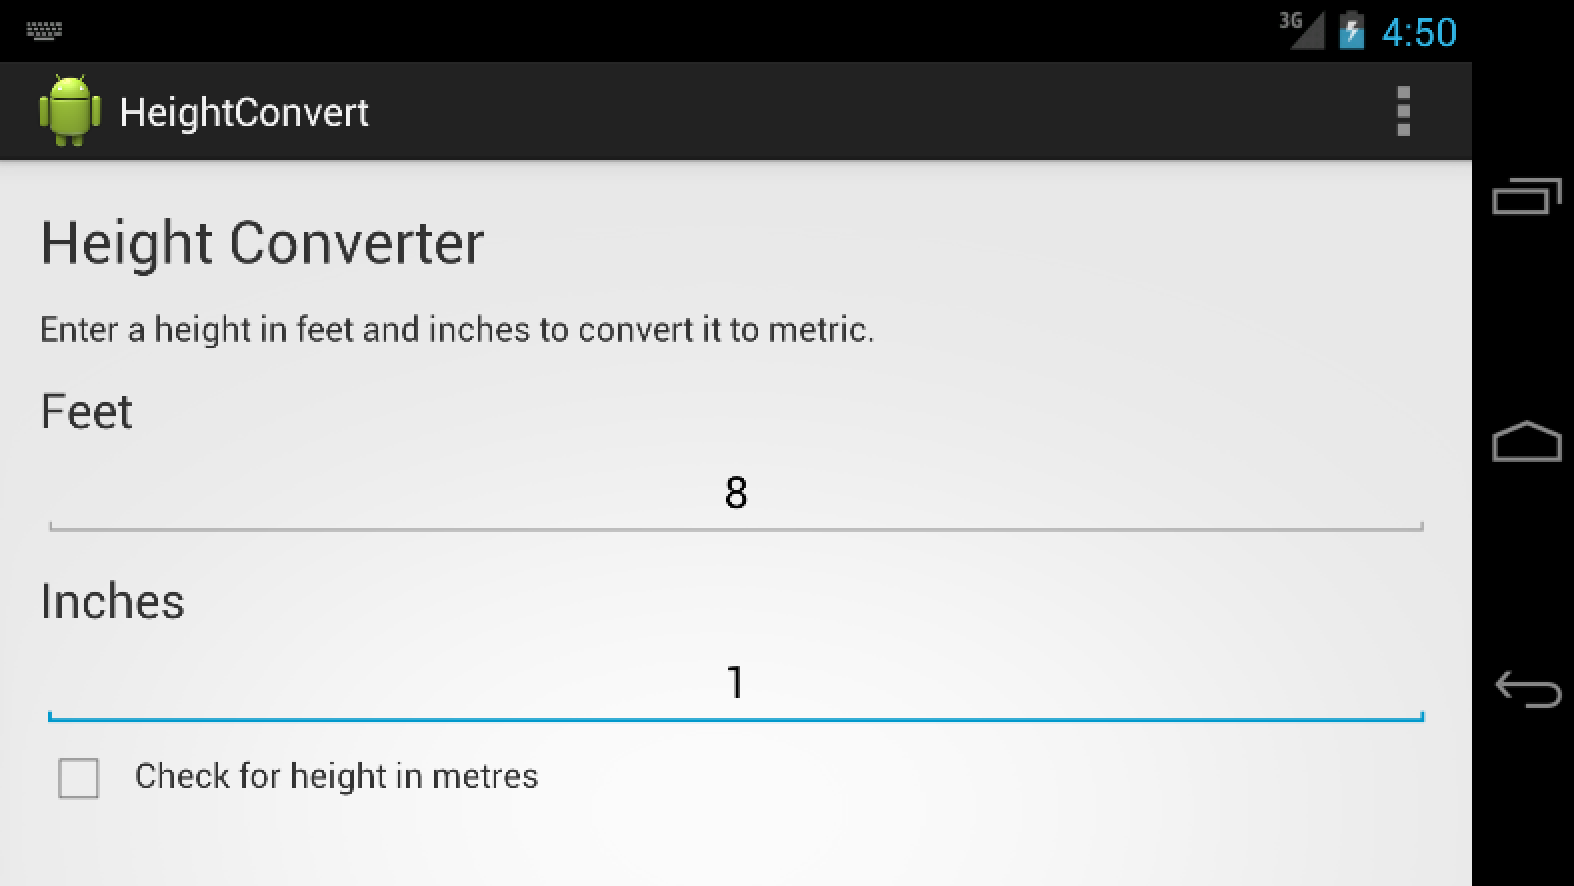
\includegraphics[width=10cm]{images/screenshot-height-landscape.png}}
}\\
\bigskip
\centering{
	\fbox{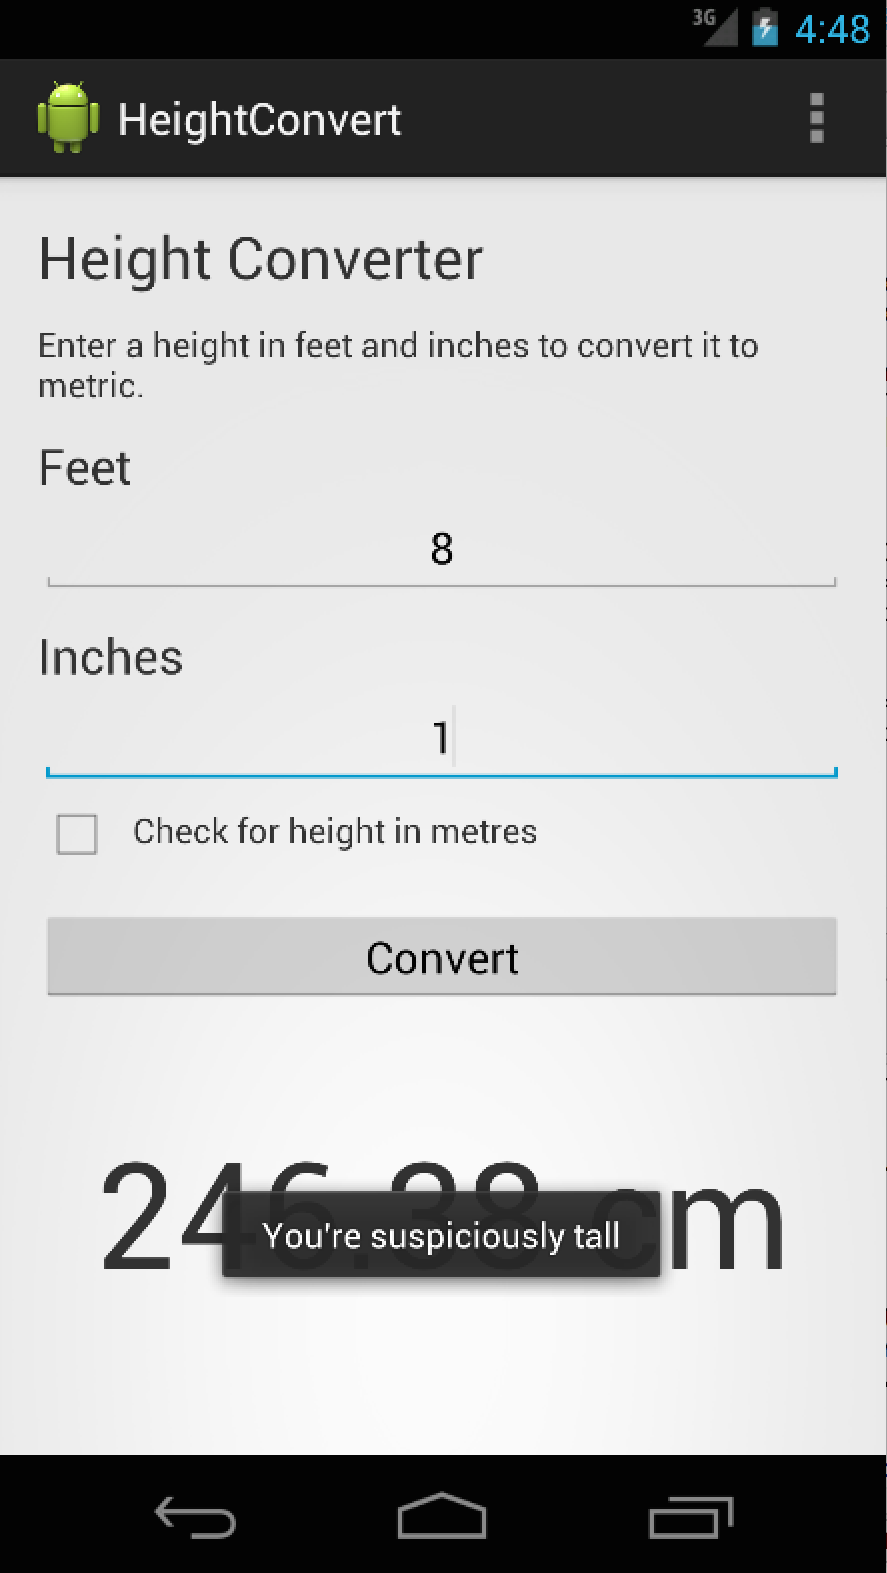
\includegraphics[width=6cm]{images/screenshot-toast.png}}
}\\
\bigskip

\subsection{Source}
\subsubsection{ConvertActivity.java}
\inputminted{java}{../../Apps/HeightConvert/app/src/main/java/au/net/danielparker/heightconvert/ConvertActivity.java}

\subsubsection{layout/activity\_convert.xml}
\inputminted{xml}{../../Apps/HeightConvert/app/src/main/res/layout/activity_convert.xml}

\subsubsection{layout-land/activity\_convert.xml}
\inputminted{xml}{../../Apps/HeightConvert/app/src/main/res/layout-land/activity_convert.xml}

\end{document}
